%=========================================
% 	   Projektmanagement					 =
%=========================================
\chapter{Projektmanagement}

Als Vorgehensmodell für das Projekt wurde ein agiles Vorgehen nach dem Vorbild von Scrum und
Extreme Programming gewählt. Dies ist hauptsächlich der Tatsache geschuldet, dass die
Verwirklichung unseres Vorhabens die Einarbeitung in zahlreiche Einzelaspekte erforderte, die
dem gesamten Team neu waren. Es war nicht abzusehen, welche Teile überhaupt umsetzbar sind
und wie erfolgreich die Implementierung verlaufen wird. Deshalb sollte das Projekt zunächst nur
den eigentlichen Stream als Kern verwirklichen und dann in kleinen Iterationen um immer mehr
Funktionalität, vor allem einer Website als User Interface, erweitert werden.

\section{Teamorganisation}
Es wurde kein Projektleiter festgelegt. Entscheidungen wurden stets im Plenum getroffen. Die
Gruppe repräsentierte sich nach außen stets gemeinsam.
Die sonstige interne Organisation des Projektteams wurde ebenfalls durch die Unwägbarkeiten der
Durchführung geprägt. Da zu Beginn noch nicht klar war, welche konkreten Aufgaben es geben
wird und wie groß ihr Umfang sein wird, konnten keine klaren Zuständigkeiten verteilt werden.
Die achtköpfige Projektgruppe teilte sich jedoch schnell in mehrere kleine Teams aus zwei oder
drei Mitgliedern, die die einzelnen Aufgaben, die sich stellten, übernahmen. So stellte sich bald
eine gewisse Spezialisierung der Teams ein. Ein „Datenbank­Team“ kümmerte sich um die
Erstellung und Pflege der Datenbank. Diese Gruppe war auch für die Installation und Wartung der
neuesten Testversion auf dem Testserver im Softwarelabor zuständig. Ein „Backend­Team“ sorgte
für den Stream und ein Interface für Nutzerabfragen aus der Datenbank. Und ein „Frontend­Team“
war für die Erstellung der Website verantwortlich. Übergreifende Aufgaben wurden von einem
vierten Team übernommen. Dazu gehörten sowohl projektorganisatorische Erledigungen
(Zeiterfassung) als auch übergreifende Aspekte der Implementierung wie etwa Sicherheitsfragen.

\section{Tools}

% [Eclipse Mars/Neon] Die Java-IDE unserer Wahl 
% [Maven] Ein Package/Buildmanager  
 
 In dem nun folgenden Abschnitt wird auf die organisatorischen Aspekte des Projekts eingegangen. Insbesondere welche Kommunikationstools und unterstützende Systeme zur erfolgreichen Durchführung des Projekts benutzt wurden.

Das Versionskontrollsystem entschied sich das Projektteam für GitHub, da einige Projektteilnehmer bereits Erfahrung mit diesem System gesammelt hatten. Außerdem erfreut es sich großer Beliebtheit im Informatik spezifischen Umfeld. Das Projekt(Code), die Datenbank und die Erstellung des Berichts wurden unter Zuhilfenahme von GitHub realisiert. Alle zusätzlichen Dokumente wie zum Beispiel Klassendiagramme, ER-Diagramme usw. wurden in einer eigens dafür angelegten Dropbox gehalten.

Als Kommunikationsplattform wurde Slack festgelegt. Dieses bietet deutliche Vorteile gegenüber Whatsapp und andern Messenger. Slack besitzt ein umfangreiches Internetforum mit unterschiedlichen Channels. Es ist sowohl möglich einzelnen Personen, sowie ganzen Gruppen oder auch allen Projektteilnehmer zu schreiben, sodass die Informationen jeden Projektteilnehmer direkt und ohne Umwege über Dritte erreichen. Slack bietet eine Integration von GitHub, Skype und Dropbox. Dadurch wird man stetig über Änderung(Commits bei GitHub) benachrichtigt. Die Benachrichtigungen sind direkt auf der Internetseite von Slack zu sehen, können aber auch über E-Mail oder die App Slack angefordert werden. Dokumente kann man sofort via Drag and Drop versenden. Auch die Umfragefunktion wurde vom Projektteam zur Terminabstimmung häufig genutzt.

Um Aufgaben besser verwalten zu können wurde das Tool Trello verwendet. Bei Trello handelt es sich um ein Tool zur dynamischen Verwaltung und Planung von verschiedenen Aufgaben. Man hat die Möglichkeit diese Aufgaben den unterschiedlichen Mitgliedern zur Bearbeitung zuzuordnen. Des weiteren kann man die einzelnen Aufgabe mit weiteren Checklisten versehen, welche die einzelnen Schritte einer Aufgabe näher erläutern. Außerdem lassen sich die Aufgaben in sogenannte Labels einteilen. Solche Labels geben das Gebiet der Aufgabe an, wie z.B. Frontend oder Datenbank.
Zuletzt werden die erstellten und personalisierten Aufgaben in einen Bereich eingeteilt, der angibt in welchem Stadium sich die Aufgabe befindet. Man unterscheidet hier zwischen den Bereichen ‘‘To Do‘‘, ‘‘In Arbeit‘‘ und ‘‘Fertig‘‘. Ist eine Aufgabe in Ihrem Bereich fertig, so wird sie einfach in den weiterführenden Bereich verschoben.

Damit der Projektaufwand genau dokumentiert werden konnte wurde eine Excel-Vorlage erstellt, welche nach jeder Kalenderwoche ausgefüllt, an eine zuvor festgelegte Person geschickt wurde. Diese fertigte eine Wochenliste an und trug die Stunden in die Gesamtliste ein. Die Wochenliste sowie die Gesamtliste wurden, sobald alle Stundenzettel eingegangen waren, erstellt und via E-Mail an den betreuenden Professor geschickt. Dadurch war eine Lückenlose Dokumentation der Stunden jedes Projektteilnehmers gewährleistet.

\begin{figure}[!h]
    \centering
    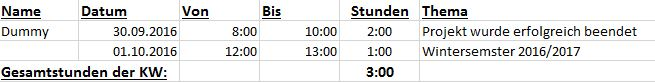
\includegraphics[width=0.85\textwidth]{Graphics/stundenzettel}
    \caption{Datensatz zum Stundenzettel}
   \label{fig:stundenzettel}
\end{figure}
 
\begin{description}	
\item [Fazit] GitHub bereitete dem Projektteam einige Probleme, da unvorhersehbare Konflikte beim Pullen, Pushen und Mergen des Projekts auftraten. Jedoch bekamen die Projektteilnehmer diese Probleme weitestgehend durch mündliche und schriftliche Abstimmung untereinander in der Griff. 

Slack wurde zur gesamten Kommunikation innerhalb des Teams benutzt. Besonders aber die Umfragefunktion, welche zur Abstimmung von Terminen sehr nützlich war. Auch um über den Fortschritt des Projekts (Commits bei GitHub) ständig informiert zu sein, war Slack bzw. die Integration von GitHub in Slack eine gute Möglichkeit. 

Trello wurde vorallem in der ersten Hälfte des Projekts benutzt. Da sich das Projektteam aber in  Gruppen für die verschiedenen Anforderungsbereiche einteilte(Frontend, Architektur und Backend), die weitestgehend unabhängig voneinander sind, gab es wenig Konflikt beim Suchen, finden und bearbeiten von Tasks. Innerhalb der Gruppen fand der Austausch vor allem über Skype statt. Dadurch gab es keine Probleme mit beispielsweise ‘‘Doppelbearbeitung‘‘ von Aufgaben. Somit war ein ergebnisorientiertes und effektives Arbeiten möglich. 
\end{description}

